\section{Preparación del entorno Linux para auditoría WiFi}

Antes de iniciar las pruebas de seguridad inalámbrica y los ataques descritos en capítulos posteriores, fue necesario preparar adecuadamente el entorno de trabajo en el sistema operativo Linux. Esta preparación tuvo como finalidad habilitar la captura, análisis y evaluación del tráfico inalámbrico mediante el uso de una antena externa compatible con modo monitor.

El entorno fue configurado exclusivamente con fines académicos, en redes propias o bajo autorización expresa, respetando los principios éticos y legales de la seguridad informática.

\subsection{Sistema operativo y herramientas utilizadas}

El sistema operativo empleado fue \textbf{Kali Linux}, seleccionado por integrar de forma nativa herramientas especializadas para auditoría de redes inalámbricas, entre las que destaca el conjunto \textit{Aircrack-ng}. Asimismo, se utilizó una antena inalámbrica basada en chipset \textbf{Atheros}, la cual permite operar en modo monitor y realizar inyección de paquetes.

\subsection{Identificación de la interfaz inalámbrica}

El primer paso consistió en identificar la interfaz de red inalámbrica reconocida por el sistema. Para ello se utilizó el comando \texttt{ifconfig}, el cual permite visualizar las interfaces disponibles y su estado actual.

\begin{lstlisting}[language=bash, caption={Identificación de interfaces de red}]
ifconfig
\end{lstlisting}

Este comando permite verificar el nombre de la interfaz inalámbrica (por ejemplo, \texttt{wlan0}) y comprobar si se encuentra en modo normal o monitor.

\subsection{Activación del modo monitor}

Una vez identificada la interfaz inalámbrica, se procedió a activar el modo monitor mediante la herramienta \texttt{airmon-ng}. El modo monitor permite capturar todos los paquetes transmitidos por el aire sin necesidad de asociarse a un punto de acceso específico.

\begin{lstlisting}[language=bash, caption={Activación del modo monitor}]
sudo airmon-ng start wlan0
\end{lstlisting}

Como resultado de este proceso, el sistema genera una nueva interfaz virtual, generalmente denominada \texttt{wlan0mon}, la cual es utilizada para las tareas de auditoría.

\subsection{Escaneo de redes inalámbricas}

Con la interfaz en modo monitor activa, se realizó un escaneo del entorno inalámbrico para identificar las redes disponibles, sus características y los dispositivos conectados. Para este propósito se utilizó la herramienta \texttt{airodump-ng}.

\begin{lstlisting}[language=bash, caption={Escaneo de redes WiFi}]
sudo airodump-ng wlan0mon
\end{lstlisting}

Este escaneo permite obtener información relevante como el BSSID, canal de operación, tipo de cifrado y estaciones asociadas a cada red.

\subsection{Captura de tráfico de una red específica}

Tras identificar la red objetivo, se configuró la captura del tráfico inalámbrico limitándola a un BSSID y canal específicos. Los paquetes capturados se almacenaron en un archivo con extensión \texttt{.cap}, el cual es indispensable para el análisis posterior.

\begin{lstlisting}[language=bash, caption={Captura de tráfico de una red específica}]
sudo airodump-ng --c 6 --bssid AA:BB:CC:DD:EE:FF -w captura wlan0mon
\end{lstlisting}

El archivo generado contiene la información necesaria para evaluar la seguridad del mecanismo de autenticación de la red.

\subsection{Forzado de reconexión mediante desautenticación}

En escenarios donde no se detecta tráfico suficiente, se recurrió a un ataque de desautenticación utilizando la herramienta \texttt{aireplay-ng}. Este procedimiento fuerza la reconexión de los clientes, permitiendo capturar el \textit{handshake} de autenticación.

\begin{lstlisting}[language=bash, caption={Ataque de desautenticación}]
sudo aireplay-ng -0 9 -a AA:BB:CC:DD:EE:FF -c 11:22:33:44:55:66 wlan0mon
\end{lstlisting}

Durante la reconexión del cliente, el \textit{handshake WPA/WPA2} queda registrado dentro del archivo \texttt{.cap}.

\subsection{Verificación de archivos capturados}

Para comprobar la correcta generación de los archivos de captura, se utilizó el comando \texttt{ls}, el cual permite listar los archivos presentes en el directorio de trabajo.

\begin{lstlisting}[language=bash, caption={Listado de archivos de captura}]
ls
\end{lstlisting}

\subsection{Análisis de seguridad mediante ataque de diccionario}

Finalmente, el archivo de captura fue analizado mediante la herramienta \texttt{aircrack-ng}, empleando un diccionario de contraseñas con el objetivo de evaluar la fortaleza de la clave de la red inalámbrica.

\begin{lstlisting}[language=bash, caption={Análisis del archivo de captura}]
sudo aircrack-ng -b AA:BB:CC:DD:EE:FF -w rockyou.txt captura-01.cap
\end{lstlisting}

El resultado del análisis permite determinar si la contraseña es robusta o vulnerable frente a ataques por diccionario.

\subsection{Desactivación del modo monitor}

Una vez finalizada la auditoría, se procedió a desactivar el modo monitor para restaurar la conectividad normal de la interfaz inalámbrica.

\begin{lstlisting}[language=bash, caption={Desactivación del modo monitor}]
sudo airmon-ng stop wlan0mon
\end{lstlisting}

\subsection{Flujo de trabajo del proceso de auditoría WiFi}

El flujo de trabajo seguido durante la auditoría inalámbrica se resume en el siguiente esquema, el cual representa la secuencia lógica desde la preparación de la interfaz hasta la obtención del resultado final.

\begin{figure}[H]
    \centering
    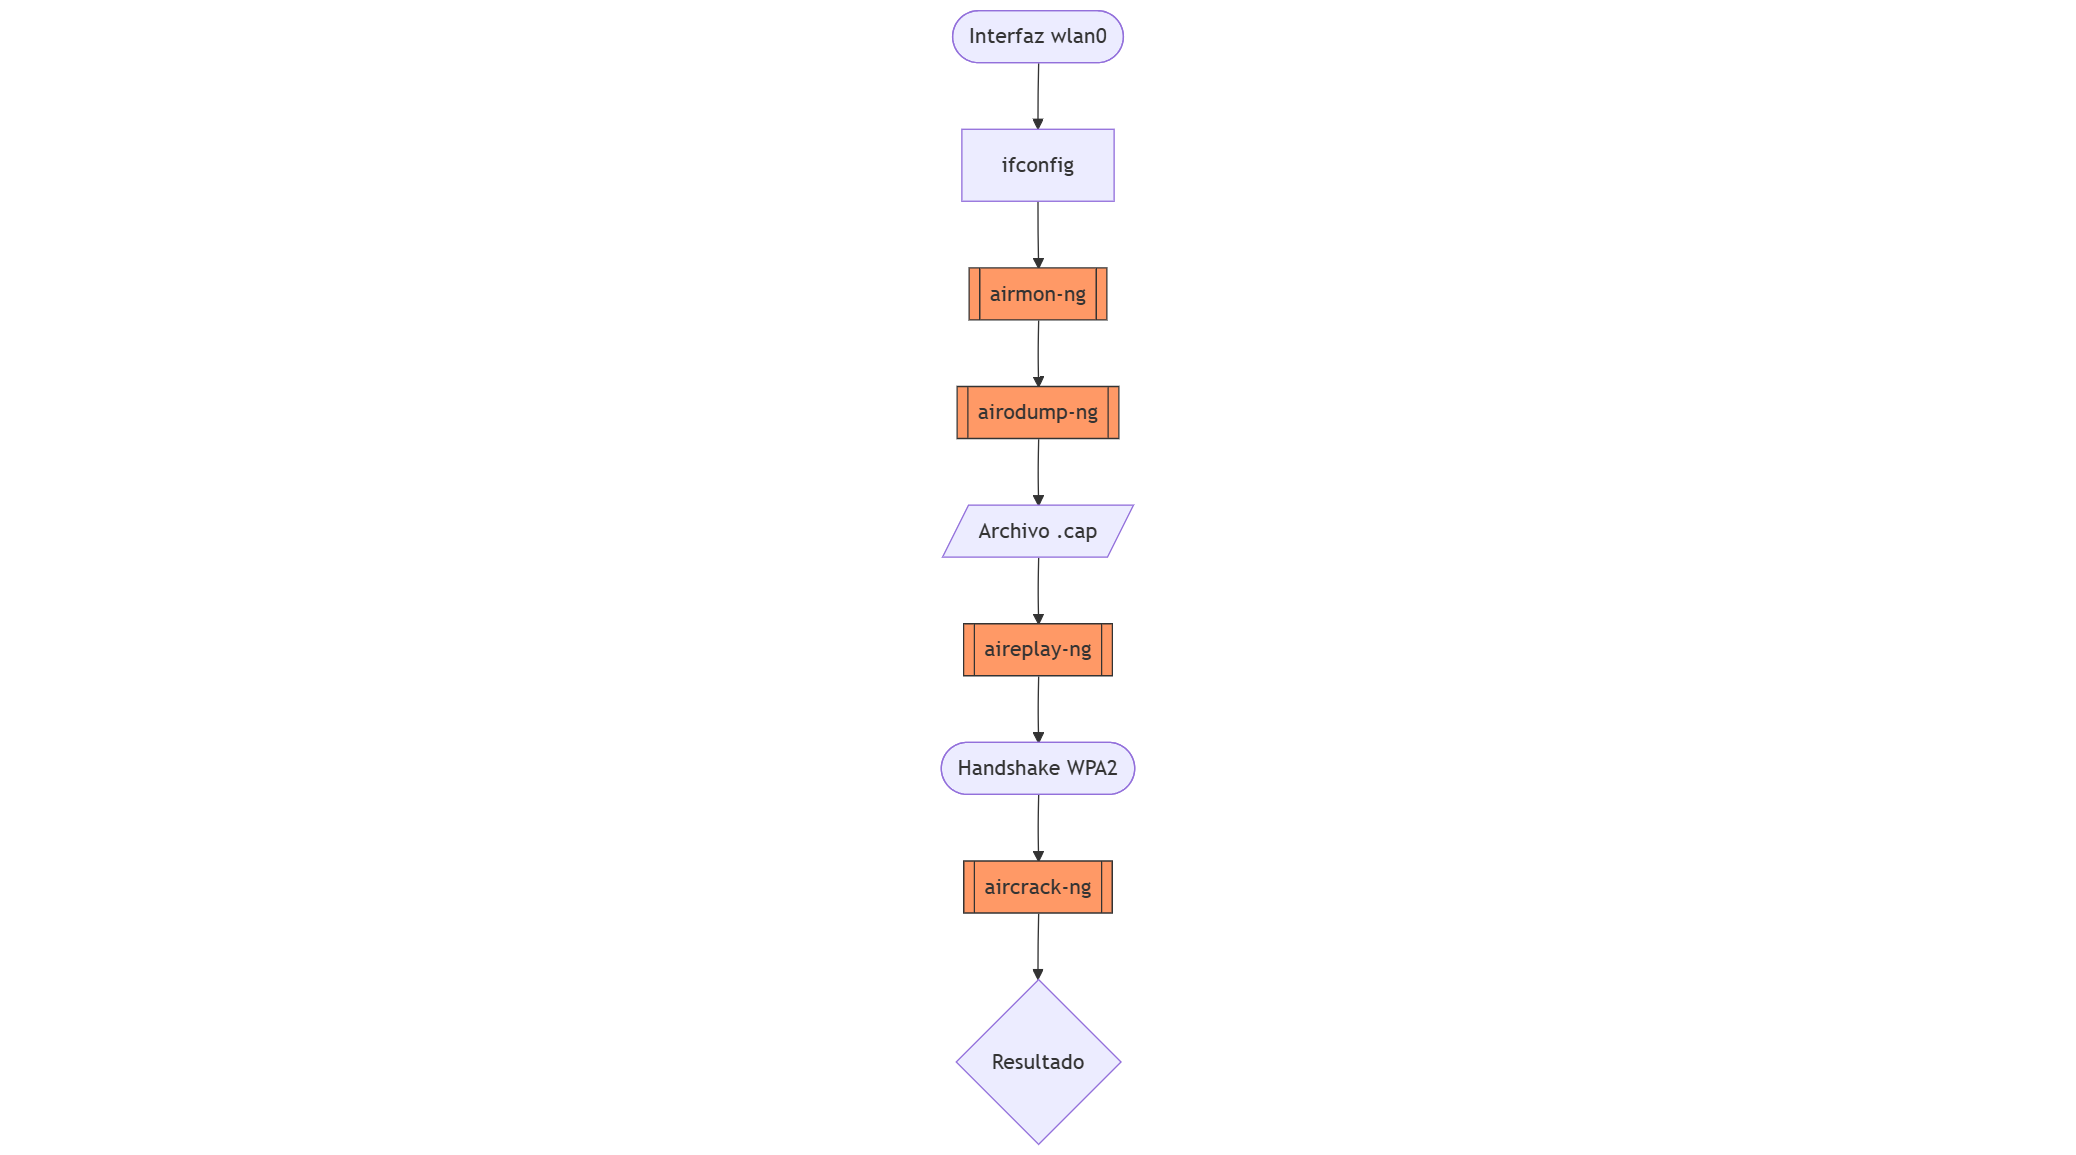
\includegraphics[width=0.9\textwidth]{assets/images/complementarios/flujo_proceso_auditoria_WiFi.png}
    \caption{Flujo de trabajo del proceso de auditoría WiFi}
    \label{fig:flujoTrabajoAuditoriaWiFi}
\end{figure}

\subsection{Importancia de la preparación del entorno}

La correcta configuración del entorno Linux y de la antena inalámbrica constituye un requisito fundamental para garantizar la validez de los resultados obtenidos. Esta fase preliminar asegura que las pruebas de seguridad se realicen de forma controlada, reproducible y alineada con los objetivos académicos del presente trabajo.
